\documentclass[problem]{mcs}

\begin{pcomments}
  \pcomment{FP_seating_around_a_round_table}
  \pcomment{by Megumi F09}
  \pcomment{edited slightly by ARM S10}
\end{pcomments}

\pkeywords{
  combinatorics
  permutation
  division rule
  inclusion-exclusion
}

%%%%%%%%%%%%%%%%%%%%%%%%%%%%%%%%%%%%%%%%%%%%%%%%%%%%%%%%%%%%%%%%%%%%%
% Problem starts here
%%%%%%%%%%%%%%%%%%%%%%%%%%%%%%%%%%%%%%%%%%%%%%%%%%%%%%%%%%%%%%%%%%%%%

\begin{problem}
  \bparts The queen and king of hearts decide to host a poker game and
  invite their best friends: the queens and kings of clubs, diamonds,
  and spades.  The queen has a round table with eight chairs labeled
  with distinct symbols $P_1, P_2, \dots, P_8$, for these
  eight people:
\begin{center}
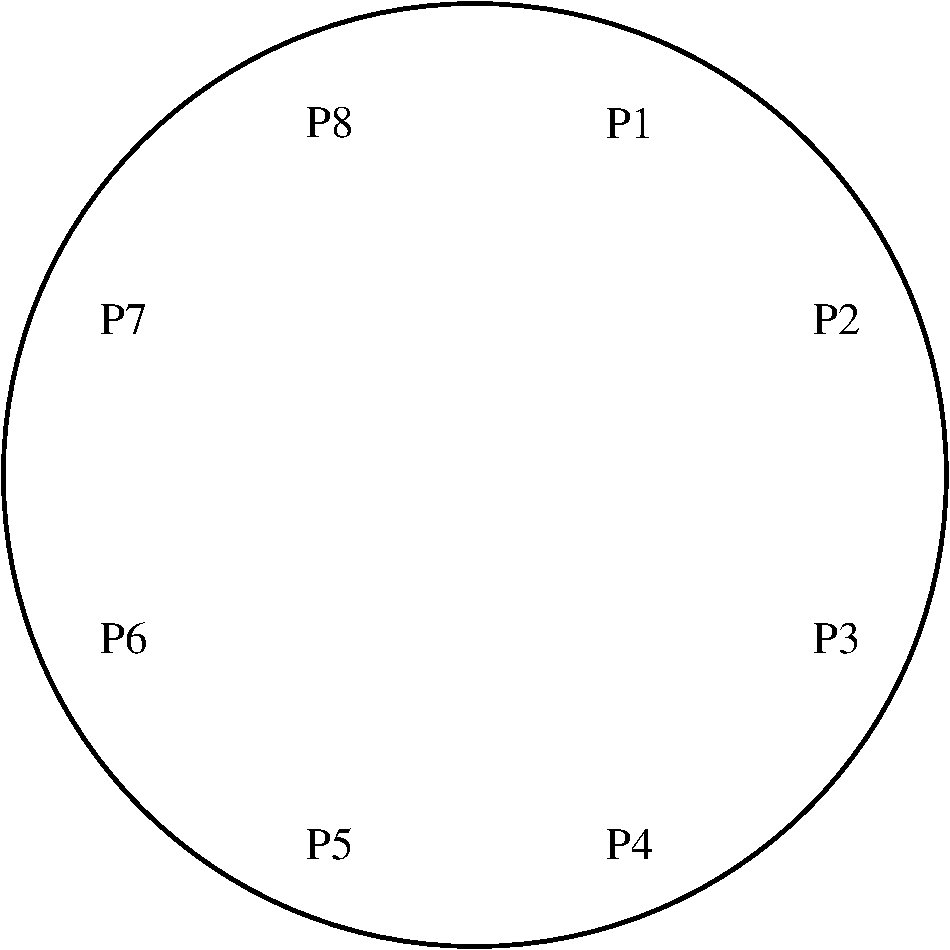
\includegraphics[height=1.5in]{figures/round_table.pdf}
\end{center}


%  for the guests (the $3$ other couples) and the host and hostess (her
%  husband and herself).
\bparts
\ppart In how many ways can the queen assign the eight people to
different chairs?

\examspace[1in]
\begin{solution}
$8!$
\end{solution}

\ppart 
\newcommand{\spa}{\spadesuit}
\newcommand{\hea}{\heartsuit}
\newcommand{\dia}{\diamondsuit}
\newcommand{\club}{\clubsuit}

A \emph{seating} is a circular arrangement of people around the table
in which all that matters is who sits next to whom, not which chairs
they are in.  In other words, two ways of assigning people to chairs
define the \emph{same seating} when one assignment is a rotation of
the other.  For example, the following two assignments of people to
chairs define the same seating. 

\begin{center}
\begin{tabular}{|l|l|l|l|l|l|l|l|}
\hline
$P_1$ & $P_2$ &$P_3$ &$P_4$ & $P_5$ & $P_6$ & $P_7$ & $P_8$ \\ \hline \hline
$K\spadesuit$ & $Q\spadesuit$ & $K\heartsuit$ & $Q\heartsuit$ & $K\diamondsuit$ & $Q\diamondsuit$ & $K\clubsuit$ & $Q\clubsuit$ \\ \hline
$K\diamondsuit$ & $Q\diamondsuit$ & $K\clubsuit$ & $Q\clubsuit$ & $K\spadesuit$ & $Q\spadesuit $ & $K\heartsuit$ & $Q\heartsuit$ \\ \hline 
\end{tabular}
\end{center}

%\begin{eqnarray*}
%K\spadesuit, Q\spadesuit, K\heartsuit, Q\heartsuit, K\diamondsuit, Q\diamondsuit, K\clubsuit, Q\clubsuit \\
%Q\heartsuit, K\diamondsuit, Q\diamondsuit, K\clubsuit, Q\clubsuit, K\spadesuit, Q\spadesuit, K\heartsuit 
%\end{eqnarray*}
%\end{definition}

\ppart How many distinct \textbf{seatings} are there?

\examspace[1.5in]
\begin{solution}
\[
\frac{8!}{8} = 7!
\]
\end{solution}

%\inhandout{\instatements{\newpage}}

\ppart How many distinct \textbf{seatings} are there if the queen and king of
hearts must be seated next to each other?
\hint Think of the king and queen as a single unit.

\examspace[1.5in]
\begin{solution}
$2! \cdot \frac{7!}{7} = 2 \cdot 6!$
\end{solution}

\ppart How many distinct \textbf{seatings} are there if the queen and
king of hearts must be seated next to each other, and the queen and
king of spades must also be seated next to each other?

\examspace[3in]
\begin{solution}
$2! \cdot 2! \cdot \frac{6!}{6} = 4 \cdot 5!$
\end{solution}

%\ppart How many distinct \textbf{seatings} are there where no one is
%seated next to their spouse?  \hint Use inclusion-exclusion. 
\ppart Briefly explain how to count the number of distinct \textbf{seatings} there are where no one is
seated next to their spouse.  \hint Use inclusion-exclusion. 

\examspace[3in]
\begin{solution}
\begin{eqnarray*}
\mbox{Answer} &=& \{\mbox{Total seatings}\} \\
&-& \binom{4}{1} \times \{\mbox{Seatings with at least one couple seated together}\} \\
&+& \binom{4}{2} \times \{\mbox{Seatings with at least two couples seated together}\} \\
&-& \binom{4}{3} \times \{\mbox{Seatings with at least three couples seated together}\} \\
&+& \binom{4}{4} \times\{\mbox{Seatings with the four couples seated together}\} \\
&=& 7! - 4 \cdot (2 \cdot 6!) + 6 \cdot (4\cdot 5!) - 4 \cdot (8 \cdot 4!) + 1 \cdot (16 \cdot 3!)
\end{eqnarray*}
\end{solution}

\eparts
\end{problem}

%%%%%%%%%%%%%%%%%%%%%%%%%%%%%%%%%%%%%%%%%%%%%%%%%%%%%%%%%%%%%%%%%%%%%
% Problem ends here
%%%%%%%%%%%%%%%%%%%%%%%%%%%%%%%%%%%%%%%%%%%%%%%%%%%%%%%%%%%%%%%%%%%%%

\endinput
